\documentclass[10pt]{article}

\usepackage[english]{babel}
\usepackage[utf8x]{inputenc}
\usepackage{amsmath}
\usepackage{graphicx}
\usepackage[colorinlistoftodos]{todonotes}
\usepackage{listings}
\usepackage{glossaries}
\usepackage{placeins}
\usepackage{fixltx2e}
\usepackage{scrpage2}
\usepackage{scrtime}
\clearscrheadfoot
\pagestyle{scrheadings}
\usepackage[
top    = 2.5cm,
bottom = 3cm,
left   = 3cm,
right  = 3cm]{geometry}
\setcounter{secnumdepth}{4}
\definecolor{dkgreen}{rgb}{0,0.6,0}
\definecolor{gray}{rgb}{0.5,0.5,0.5}
\definecolor{mauve}{rgb}{0.58,0,0.82}

\newcommand{\executeiffilenewer}[3]{%
\ifnum\pdfstrcmp{\pdffilemoddate{#1}}%
{\pdffilemoddate{#2}}>0%
{\immediate\write18{#3}}\fi%
}
\newcommand{\includesvg}[1]{%
\executeiffilenewer{#1.svg}{#1.pdf}%
{inkscape -z -D --file=#1.pdf --export-pdf=#1.pdf --export-latex}%
\input{#1.pdf_tex}%
}

\lstset{frame=tb,
  language=Java,
  aboveskip=3mm,
  belowskip=3mm,
  showstringspaces=false,
  columns=flexible,
  basicstyle={\small\ttfamily},
  numbers=none,
  numberstyle=\tiny\color{gray},
  keywordstyle=\color{blue},
  commentstyle=\color{dkgreen},
  stringstyle=\color{mauve},
  breaklines=true,
  breakatwhitespace=true
  tabsize=3
}


\begin{document}


\begin{titlepage}
\begin{center}
% Oberer Teil der Titelseite:

%NEEDS TO BE OUT COMMENTED sometimes
%\includegraphics[width=1.0\textwidth]{../../pictures/robonavlogo}\\  

\includegraphics[width=0.5\textwidth]{pictures/logo}\\  

\LARGE TGM - HTBLuVA Wien XX \\ Informationstechnologie  \\[1.5cm]

% Title
\rule{14cm}{1mm}
{ \huge \bfseries \\[0.4cm]  \huge Haidn \& Siegel \\ \LARGE Backup with Mysql and Postgresql \\[0.4cm] }

\rule{14cm}{1mm}
\noindent 

\vspace{7cm}
\small
\begin{center}
  \begin{tabular}{ | p{0.1\textwidth} | p{0.2\textwidth} | p{0.2\textwidth} | p{0.1\textwidth} | p{0.2\textwidth} |}
    \hline
\textbf{Version} & \textbf{Autor} & \textbf{Datum} & \textbf{Status} & \textbf{Kommentar} \\ 
    \hline 
    \hline
0.1 & Siegel & 2014.11.28 & Draft &    \\ 
0.2 & Haidn & 2014.12.09 & Draft &  Mysql finished  \\ 
0.3 & Siegel & 2014.12.14 & Draft &  Postgres finished  \\ 
1.1 & Haidn & 2014.12.15 & Finished &  QA done  \\ 

    \hline
  \end{tabular}
\end{center}

\vfill

% Bottom of the page
{\small Version of this document: \today ~at  \thistime    }
\end{center}

%\end{center}
\end{titlepage}


%HEADER AND FOOTER
\pagenumbering{arabic}
\ohead{\headmark}
\ifoot{© Haidn, Siegel}
\ofoot{\pagemark}
\tableofcontents

\section{Working time}
\subsection{Estimated}
\begin{table}[h]

\begin{tabular}{|p{0.5\textwidth}|p{0.2\textwidth}|p{0.2\textwidth}|}
\hline
\textbf{Task}    & \textbf{Person}                                               & \textbf{Time in hours                              } \\ \hline \hline
Setting up the Databases & \begin{tabular}[c]{c} Haidn \\Siegel\end{tabular} & \begin{tabular}[c]{c}0.5\\ 0.5\end{tabular}    \\ \hline 
Getting some informations about backups & \begin{tabular}[c]{c} Haidn \\Siegel\end{tabular} & \begin{tabular}[c]{c}1\\ 1\end{tabular}    \\ \hline 
mysqldump & \begin{tabular}[c]{c} Haidn \\Siegel\end{tabular} & \begin{tabular}[c]{c}1\\ 1\end{tabular}    \\ \hline 
mysqlbackup & \begin{tabular}[c]{c} Haidn \\Siegel\end{tabular} & \begin{tabular}[c]{c}1\\ 1\end{tabular}    \\ \hline 
system-level commands & \begin{tabular}[c]{c} Haidn \\Siegel\end{tabular} & \begin{tabular}[c]{c}1\\ 1\end{tabular}    \\ \hline 
mysqlhotcopy & \begin{tabular}[c]{c} Haidn \\Siegel\end{tabular} & \begin{tabular}[c]{c}1\\ 1\end{tabular}    \\ \hline 
Automated Backup & \begin{tabular}[c]{c} Haidn \\Siegel\end{tabular} & \begin{tabular}[c]{c}1\\ 1\end{tabular}    \\ \hline 
Documentation & \begin{tabular}[c]{c} Haidn \\Siegel\end{tabular} & \begin{tabular}[c]{c}0.5\\ 0.5\end{tabular}    \\ \hline 
pg\_dump & \begin{tabular}[c]{c} Haidn \\Siegel\end{tabular} & \begin{tabular}[c]{c}2\\ 2\end{tabular}    \\ \hline 
pg\_restore & \begin{tabular}[c]{c} Haidn \\Siegel\end{tabular} & \begin{tabular}[c]{c}1\\1\end{tabular}    \\ \hline 
automated postgres & \begin{tabular}[c]{c} Haidn \\Siegel\end{tabular} & \begin{tabular}[c]{c}2\\2\end{tabular}    \\ \hline 
\hline \hline
Total & \begin{tabular}[c]{c}Haidn\\ Siegel\end{tabular} & \begin{tabular}[c]{c}12\\12\end{tabular}   \\ \hline 
\textbf{Total Team} & & \textbf{21.5 hours}  \\ \hline 
\end{tabular}
\end{table}
\newpage
\subsection{Final}
\begin{table}[h]

\begin{tabular}{|p{0.5\textwidth}|p{0.2\textwidth}|p{0.2\textwidth}|}
\hline
\textbf{Task}    & \textbf{Person}                                               & \textbf{Time in hours                              } \\ \hline \hline
Setting up the Databases & \begin{tabular}[c]{c} Haidn \\Siegel\end{tabular} & \begin{tabular}[c]{c}1\\ 1\end{tabular}    \\ \hline 
Getting some informations about backups & \begin{tabular}[c]{c} Haidn \\Siegel\end{tabular} & \begin{tabular}[c]{c}2\\ 1\end{tabular}    \\ \hline 
mysqldump & \begin{tabular}[c]{c} Haidn \\Siegel\end{tabular} & \begin{tabular}[c]{c}2\\ 2\end{tabular}    \\ \hline 
mysqlbackup & \begin{tabular}[c]{c} Haidn \\Siegel\end{tabular} & \begin{tabular}[c]{c}0\\ 2\end{tabular}    \\ \hline 
system-level commands & \begin{tabular}[c]{c} Haidn \\Siegel\end{tabular} & \begin{tabular}[c]{c}2\\ 0\end{tabular}    \\ \hline 
mysqlhotcopy & \begin{tabular}[c]{c} Haidn \\Siegel\end{tabular} & \begin{tabular}[c]{c}1.5\\ 1.5\end{tabular}    \\ \hline 
Automated Backup & \begin{tabular}[c]{c} Haidn \\Siegel\end{tabular} & \begin{tabular}[c]{c}1.5\\ 2\end{tabular}    \\ \hline 
Documentation Mysql & \begin{tabular}[c]{c} Haidn \\Siegel\end{tabular} & \begin{tabular}[c]{c}1\\ 2\end{tabular}    \\ \hline 
pg\_dump & \begin{tabular}[c]{c} Haidn \\Siegel\end{tabular} & \begin{tabular}[c]{c}2\\ 2\end{tabular}    \\ \hline 
pg\_restore & \begin{tabular}[c]{c} Haidn \\Siegel\end{tabular} & \begin{tabular}[c]{c}0.5\\ 0.5\end{tabular}    \\ \hline 
Documentation Postgres & \begin{tabular}[c]{c} Haidn \\Siegel\end{tabular} & \begin{tabular}[c]{c}1\\ 1\end{tabular}    \\ \hline 
Automated Postgres Backup & \begin{tabular}[c]{c} Haidn \\Siegel\end{tabular} & \begin{tabular}[c]{c}1.5\\ 1.5\end{tabular}    \\ \hline 

\hline \hline
Total & \begin{tabular}[c]{c}Haidn\\ Siegel\end{tabular} & \begin{tabular}[c]{c}16\\15.5\end{tabular}   \\ \hline 
\textbf{Total Team} & & \textbf{31.5 hours}  \\ \hline 
\end{tabular}
\end{table}
\FloatBarrier
Therefore it took us a little bit longer (about 10 hours more).
\newpage
\section{Working situation}
\subsection{Database models}
We were using the create scripts from the last VSDB homework. In this we had done two similar create scripts using both mysql and postgres. \\ The database contains triggers and inserts for each table.\\ The ER can be seen in figures \ref{mysqler} and \ref{pger}.
\begin{figure}[!h]
	\begin{center}
		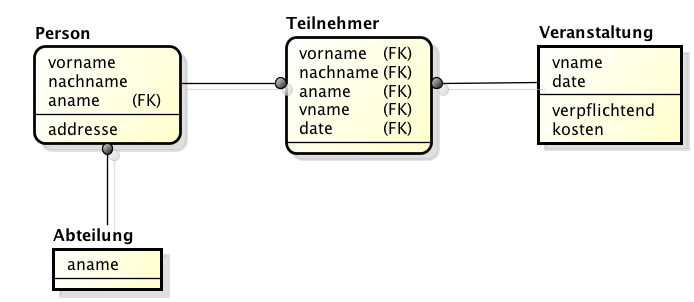
\includegraphics[width=0.8\linewidth]{pictures/ERD_mysql}
		\caption{Entity Relationship Diagram for the mysql database}
		\label{mysqler}
	\end{center}
\end{figure}
\begin{figure}[!h]
	\begin{center}
		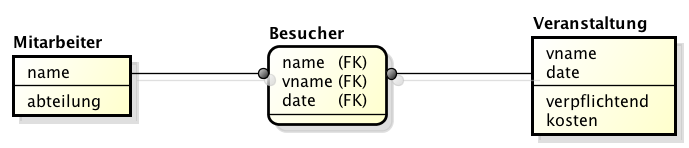
\includegraphics[width=0.8\linewidth]{pictures/ERD_psql}
		\caption{Entity Relationship Diagram for the postgres database}
		\label{pger}
	\end{center}
\end{figure}
\FloatBarrier
\subsection{Hannah}
Databases: Mysql Version 14.14, Distribution 5.5.40, PostgreSQL 9.3.5\\
DB-Server Environment (VM) :  Ubuntu 14.04 LTS , it's IP: 192.168.117.131
\subsection{Martin}
Database: Mysql Version 14.14 Distribution 5.5.31\\
DB-Server Environment (VM) : Linux Debian 3.10.11-1
\newpage
\newpage
\section{Backups general}
\subsection{Why should backups be done?}
After a drop-out, a recovery must me done. \\
To avoid a loss of data, a backup must be done before an drop-out occurs and it always should be current. \\ \\
Backups are not only needed for recovery purposes, but also for archival storage purposes.
\subsection{Logical versus physical backups}
Logical backups save information represented as logical database structure (e.g. \texttt{Create Database}, \texttt{Create Table}  statements) and content (e.g \texttt{Insert} statements). Physical backups consist of raw copies of the directories and files that store database contents. \\ \\
Logical backups :
\begin{enumerate}
\item Backup is done by querying the MySQL server
\item Slower than physical methods
\item Output is larger than physical methods
\item The Backup and the Restore can be done either for all databases (server level), only for one database (database level) or only for specific tables (table level)
\item Doesent include log or config files
\item Backups are mostly done with the database still running
\item Can be easily imported
\item Backups stored in logical format are machine independent!
\end{enumerate}\cite{mysqlbackupandrectypesman}
\\ \\Physical backups :
\begin{enumerate}
\item Exact copy of database files which are stored on the disk
\item Output is more compact than logical ones
\item The granularity of the data that can be stored depends on the engine (e.g. InnoDb shares files with other tables..) 
\item Can include log or config files
\item Backups stored in logical format are machine dependent!
\item Backups are seldom done with the database running, and if then the database files must be locked.
\item Can be easily imported
\end{enumerate} \cite{mysqlbackupandrectypesman}
\subsection{Full versus incremental backups}
"Some file system implementations enable “snapshots” to be taken. These provide logical copies of the file system at a given point in time, without requiring a physical copy of the entire file system. [..] MySQL itself does not provide the capability for taking file system snapshots. It is available through third-party solutions such as Veritas, LVM, or ZFS.", \cite{mysqlbackupandrectypesman}
\\ \
"A full backup includes all data managed by a MySQL server at a given point in time. An incremental backup consists of the changes made to the data during a given time span (from one point in time to another). MySQL has different ways to perform full backups, such as those described earlier in this section. Incremental backups are made possible by enabling the server's binary log, which the server uses to record data changes. \\
Incremental recovery is recovery of changes made during a given time span. This is also called point-in-time recovery because it makes a server's state current up to a given time. Point-in-time recovery is based on the binary log and typically follows a full recovery from the backup files that restores the server to its state when the backup was made. Then the data changes written in the binary log files are applied as incremental recovery to redo data modifications and bring the server up to the desired point in time.", \cite{mysqlbackupandrectypesman}
%\textbf{Komplettsicherung} 
%Alle Daten jedes mal 
% \textbf{Differenzsicherung}
% nur die Aenderungen werden abgespeichert
%\textbf{Inkrementelle Sicherung} 
%- Alles und alle Aenderungen
%(Aenderungen 1, 2, 3, … werden abgespeichert und muessen in der richtigen Reihenfolge eingespeichert werden)
\subsubsection{Online versus Offline backups}
Online backups, also called hot backups, take place while the server is running so that the database can still be used.\\
Offline backups, also called cold backups, take place while the server is not running and therefore the database is not availiable. \\ \\
Online backups :
\begin{enumerate}
\item Clients can still access the database
\item The backup must be made carefully, in order to secure, that the clients have not changed informations in the mean time that could compromise the backup's integrity
\end{enumerate} \cite{mysqlbackupandrectypesman}\\ \\
Offline backups :
\begin{enumerate}
\item Clients can not access the database
\item The backup is easier
\end{enumerate}
A similar distinction between online and offline applies for recovery operations.
 \cite{mysqlbackupandrectypesman}
\newpage
\section{Mysql Backup}
\subsection{Logical Backup into Files with mysqldump}
Mysql has an option called mysqldump. Mysql dump can connect to local or remote servers.\cite{mysqlbackupandrectypesman}
\subsubsection{Performing a database dump}
To do a backup from only one database, the following command needs to be executed: \\
\texttt{ mysqldump -u [user] -p [database\_name] \textgreater ~dumpfilename.sql } \\
After typing in the password, a file will be available which, in this case is called \texttt{dumpfilename.sql}.\\ 
The content of the dumpfile is the following:
\begin{lstlisting}    
-- MySQL dump 10.13  Distrib 5.5.40, for debian-linux-gnu (x86_64)
--
-- Host: localhost    Database: insy1
-- ------------------------------------------------------
-- Server version	5.5.40-0ubuntu0.14.04.1

/*!40101 SET @OLD_CHARACTER_SET_CLIENT=@@CHARACTER_SET_CLIENT */;
/*!40101 SET @OLD_CHARACTER_SET_RESULTS=@@CHARACTER_SET_RESULTS */;
/*!40101 SET @OLD_COLLATION_CONNECTION=@@COLLATION_CONNECTION */;
/*!40101 SET NAMES utf8 */;
/*!40103 SET @OLD_TIME_ZONE=@@TIME_ZONE */;
/*!40103 SET TIME_ZONE='+00:00' */;
/*!40014 SET @OLD_UNIQUE_CHECKS=@@UNIQUE_CHECKS, UNIQUE_CHECKS=0 */;
/*!40014 SET @OLD_FOREIGN_KEY_CHECKS=@@FOREIGN_KEY_CHECKS, FOREIGN_KEY_CHECKS=0 */;
/*!40101 SET @OLD_SQL_MODE=@@SQL_MODE, SQL_MODE='NO_AUTO_VALUE_ON_ZERO' */;
/*!40111 SET @OLD_SQL_NOTES=@@SQL_NOTES, SQL_NOTES=0 */;

--
-- Table structure for table `Abteilung`
--

DROP TABLE IF EXISTS `Abteilung`;
/*!40101 SET @saved_cs_client     = @@character_set_client */;
/*!40101 SET character_set_client = utf8 */;
CREATE TABLE `Abteilung` (
  `aname` varchar(255) NOT NULL,
  `sync_state` enum('current','old','new','syncing','deleting') NOT NULL DEFAULT 'new',
  PRIMARY KEY (`aname`,`sync_state`)
) ENGINE=InnoDB DEFAULT CHARSET=latin1;
/*!40101 SET character_set_client = @saved_cs_client */;
...
\end{lstlisting}    
Even trough that in this case there is only one create table command, there is a lot of bulk. \\
In the next example, the Inserts into a table can be seen, and here it actually is not too much bulk.
Still, whenever saving a database dump like this, the file will be quite big, which might be a big disadvantage! 
\begin{lstlisting}    
INSERT INTO `Person` VALUES 
('Aly','Ahmed','Facility Management','Doppelte gasse','current'),
('Dominik','Scholz','IT','Schwarze gasse','current'),
('Elias','Frantar','Kindergarten','Heiligenstadt gasse','current'),
('Hannah','Siegel','HR','Max Kahrer gasse','current'),
('Jakob','Saxinger','Kueche','Max Soundso gasse','current'),
('Martin','Haidn','Managment','Gruene gasse','current'),...
\end{lstlisting}    
\textbf{Backup of only one table using mysqldump}\\
\texttt{ mysqldump -u  [user] -p [database\_name] [table\_name] \textgreater ~dumpfilename.sql } \\ \\
\textbf{Backup of more than one database using mysqldump}\\
\texttt{ mysqldump -u  [user] -p --databases [database\_name1] [database\_name2] \textgreater ~dumpfilename.sql } \\ 
\textbf{Backup of all databases using mysqldump}\\
\texttt{ mysqldump -u  [user] -p --all-databases \textgreater ~dumpfilename.sql } \\ \\
\textbf{Backup of only the structure without any data}\\
\texttt{mysqldump -u  [user] -p [-d|--no-data] [database\_name] \textgreater ~dumpfilename.sql }
\subsubsection{Drop statements}
If drop-statements should be added, the following parameters can simply be added:
\begin{table}[h]
\begin{tabular}{ll}
\textbf{Format}     & \textbf{Description}                                                \\
--add-drop-database & Adds a DROP DATABASE statement before each CREATE DATABASE statement \\
--add-drop-table    & Adds a DROP TABLE statement before each CREATE TABLE statement       \\
\end{tabular}
\end{table} \cite{mysqldumpman}
The option \texttt{--add-drop-trigger} was supported in version 5.1, but it is not availiable anymore in 5.5:  
\begin{lstlisting}    
root@ubuntu:/var/lib/mysql# mysqldump -u root -p insy2 --add-drop-trigger > df1.sql
mysqldump: unknown option '--add-drop-trigger' 
\end{lstlisting}    
Weirdly, even trough we didn't add the \texttt{--add-drop-table} command in the first place, the dump includes the 
\texttt{DROP TABLE IF EXISTS} Command, as it can be seen in the first code snippet under this section:
\begin{lstlisting}    
DROP TABLE IF EXISTS `Abteilung`;
\end{lstlisting}    

\subsubsection{Performing a data restore}
After having dropped the database, the following commad was restoring the data. this has worked out fine:
To do a backup from only one database, the following command needs to be executed: \\
\texttt{mysql -u root -p [database\_name] \textless dumpfilename.sql} \\ \\
With this type of recovery, even the triggers have been imported.
\newpage
\subsection{Physical backup with mysqlbackup}
A physical backup tool is available in the mysql Enterprise Edition. These information could be found under \cite{mysqlenterprisebackup}.
Of course, it might not be the most trustful source, because mysql will surely try to promote it's product, but still it might be about that much faster:
\begin{figure}[!h]
	\begin{center}
		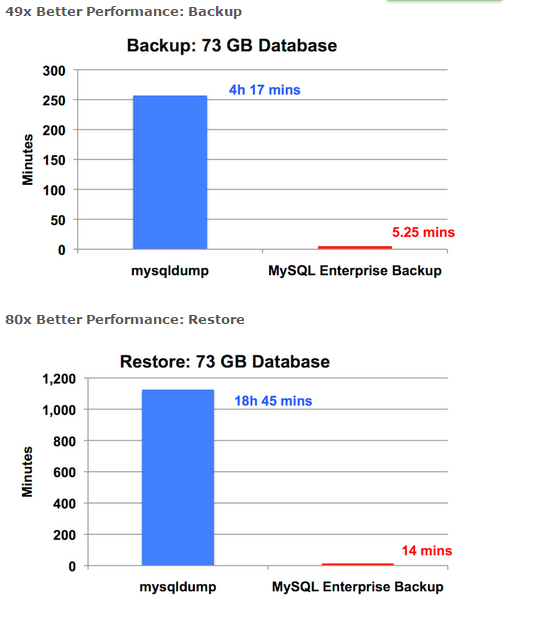
\includegraphics[width=0.7\linewidth]{pictures/mysqlentbackup}
		\caption{Difference between mysqlbackup and mysqldump }
		\label{differenceent}
	\end{center}
\end{figure}\FloatBarrier
\subsection{Restoring from another Database}
Also, a database could be copied from another using these commands.
We have tried this out an it worked.\cite{so1}
\begin{lstlisting}    
MyISAM:
CREATE TABLE db2.mytable LIKE db1.mytable;
ALTER TABLE db2.mytable DISABLE KEYS;
INSERT INTO db2.mytable SELECT * FROM db1.mytable;
ALTER TABLE db2.mytable ENABLE KEYS;
 \end{lstlisting}    
 \begin{lstlisting}    
INNODB:
CREATE TABLE db2.mytable LIKE db1.mytable;
INSERT INTO db2.mytable SELECT * FROM db1.mytable;
  \end{lstlisting}    
\subsection{Physical backup using File system commands}
\label{sec:cpmysql}
In Order to copy the files, the location must be found out. This can be done with the \texttt{select @@datadir} command within mysql.
\begin{figure}[!h]
	\begin{center}
		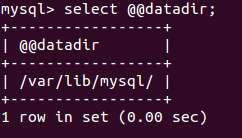
\includegraphics[width=0.4\linewidth]{pictures/datadir_mysql}
		\caption{Output of the select @@datadir command}
		\label{differenceent}
	\end{center}
\end{figure}
\FloatBarrier
In figure \ref{content}, the content of the insy1 database can be seen. The only MyISAM table is 'Logged'.\\
Also, each trigger has its own file.
\FloatBarrier
\begin{figure}[!h]
	\begin{center}
		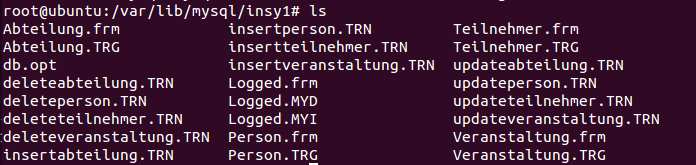
\includegraphics[width=0.8\linewidth]{pictures/ls_mysql_insy1}
		\caption{Content of the ver/etc/mysql folder}
		\label{content}
	\end{center}
\end{figure}
\FloatBarrier
\subsubsection{MyISAM}
Copying files when using a MyISAM Database, is possible, because every Table maps to exactly one file. \\
"However, you cannot just move the .frm. You must move all components.", \cite{so1} \\
There are three files (see also in figure \ref{content}) which have something to do with the table:
\begin{itemize}
\item /var/lib/mysql/insy1/Logged.frm
\item /var/lib/mysql/insy1/Logged.MYD (Table Database)
\item /var/lib/mysql/insy1/Logged.MYI (Table Indexes)
\end{itemize}
When simply coping these files, dropping the table and coping them back, \\ and then calling a \texttt{Select * from Logged} command, the following error message occurs:
\begin{lstlisting}
 ERROR 1017 (HY000): Can't find file: './insy1/Logged.frm' (errno: 13)
\end{lstlisting}
When searching for a solution, there are some, but mostly it says that it is really better backing mysql databases up with \texttt{mysqlhotcopy}.
\subsubsection{InnoDB}
On the other hand, doing a backup when coping files, is "risky (near suicidal) with InnoDB.",\cite{so1}
Therefore, whenever using InnoDB, a backup should be done with \texttt{mysqldump}.
\subsection{mysqlhotcopy}
"mysqlhotcopy is a Perl script that was originally written and contributed by Tim Bunce. It uses FLUSH TABLES, LOCK TABLES, and cp or scp to make a database backup. It is a fast way to make a backup of the database or single tables, but it can be run only on the same machine where the database directories are located. mysqlhotcopy works only for backing up MyISAM and ARCHIVE tables. It runs on Unix.",\cite{mysqlhotcopyman}
\subsubsection{Copying the files}
Using the mysqlhotcopy is a really easy way to copy the files. In the following example, it can be seen, what command must be used and the output. \\
\begin{lstlisting}
hsiegel@ubuntu:~/Documents/sync_het_db/Create$ sudo /usr/bin/mysqlhotcopy -u root -p secret_password insy1 /home/hsiegel/Desktop --allowold --keepold
Flushed 5 tables with read lock (`insy1`.`Abteilung`, `insy1`.`Logged`, `insy1`.`Person`, `insy1`.`Teilnehmer`, `insy1`.`Veranstaltung`) in 0 seconds.
Locked 0 views () in 0 seconds.
Copying 24 files...
Copying indices for 0 files...
Unlocked tables.
mysqlhotcopy copied 5 tables (24 files) in 0 seconds (0 seconds overall).
\end{lstlisting}
This simply copies the files from /var/lib/mysql/insy1 to the source destination.
\begin{figure}[!h]
	\begin{center}
		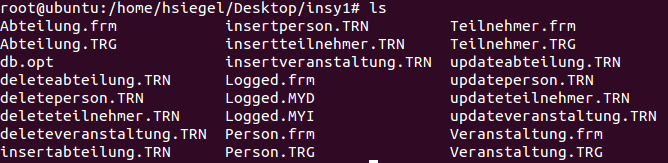
\includegraphics[width=0.8\linewidth]{pictures/lsdesktop}
		\caption{Content of the insy1 folder, which has been generated using mysqlhotcopy}
		\label{content}
	\end{center}
\end{figure}

\subsubsection{Restoring}
"To restore the backup from the mysqlhotcopy backup, simply copy the files from the backup directory to the /var/lib/mysql/{db-name} directory. Just to be on the safe-side, make sure to stop the mysql before you restore (copy) the files. After you copy the files to the /var/lib/mysql/{db-name} start the mysql again.",\cite{mysqlhtcoptut}
In our example, restoring after having done a mysqlhotcopy didn't work either, with the same error message as before:
\begin{lstlisting}
 ERROR 1017 (HY000): Can't find file: './insy1/Logged.frm' (errno: 13)
\end{lstlisting}
\subsection{Backup of Triggers / Stored Routines}
When using mysqldump, the triggers have been saved automatically and the import has not been a problem. \\
Because the mysqlhotcopy didn't work, we couldn't evaluate it by our selves if the triggers were restored. But normally, it should be possible using mysqlhotcopy as well.

\subsection{Online Backup}
With MySQL Enterprise Backup, a hot backup is possible. \\
Also, mysqlhotcopy, as the name already says, is also able to perform hot backups, because the Perl script handles the locking.
Mysqldump is executing Select statements on the database, therefore it is a hot copy as well, but in this case, it might be really slow for users and the task itself.
\subsection{Remote Backups}
\subsubsection{Using mysqldump to perform remote backups}
You can specify the server name as an option to mysqldump: 
\texttt{mysqldump --host [server\_name] [database\_name] \textgreater ~dumpfilename.sql}
\subsubsection{Using ftp to perform remote backups}
As described in section \ref{sec:cpmysql}, the files can simply be copied, and this process of copying can also be performed using ftp.
\subsection{Automated Backups}
An important way of performing backups is that they can also be automatised. This has the advantage, that the administrator doesn't has to think about doing a backup and therefore is not able to forget it, and also backups can then be scheduled at times, when the database server might not be very busy, so the backup is faster and the client do not notice that a backup task has just been performed.  \\
Automised Backups with mysql are quite easy. This can be done using the tool automysqlbackup. \\
The following commands have to be done: \\
\texttt{sudo apt-get install automysqlbackup} \\
\texttt{sudo automysqlbackup} \\ \\
The main configuration file for automysqlbackup is located at \texttt{/etc/default/automysqlbackup}. \\
"If you only want to back up certain databases, you can specify them in the DBNAMES configuration variable. Conversely, if you want to backup everything except certain databases, you can use the DBEXCLUDE configuration variable to list what to exclude.",\cite{sceduleddbbck} \\
The backups will be located at \texttt{/var/lib/automysqlbackup}. There are three folders: \texttt{daily, weekly, monthly}.
The automised backup worked, in my daily folder, each day there is a new File.\\
"By default, the daily folder will contain all of the last seven days. The weekly folder will grow to contain the database as it was on Sunday each of the last fifty-two weeks. Similarly, monthly will contain the end of all each of the last twelve months.",\cite{sceduleddbbck}
\begin{figure}[!h]
	\begin{center}
		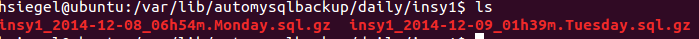
\includegraphics[width=1.0\linewidth]{pictures/mysql_autobackup}
		\caption{Content of the \texttt{/var/lib/automysqlbackup} folder with two automised backups}
		\label{content}
	\end{center}
\end{figure}
\FloatBarrier
\subsubsection{Backup at a certain time}
Because we couldn't find the possibility to set a time when the backup should be done with the automysqlbackup option, we looked further. \\
There is the possibility to use the cron-deamon. This is a program which can execute shell scripts automatically.
All that had to be done, was adding a line into the cron-table. \\
This can be done using the \texttt{crontab -e} command. \\
In figure \ref{fig:crontab} the crontab syntax is described. We added the following line:
\begin{lstlisting}
15 20 * * *   /usr/sbin/automysqlbackup
\end{lstlisting}
\begin{figure}[!h]
	\begin{center}
		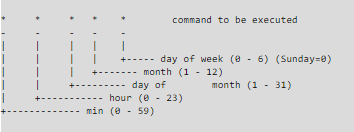
\includegraphics[width=1.0\linewidth]{pictures/crontab}
		\caption{Usage of the crontab file\cite{crontabref}}
		\label{fig:crontab}
	\end{center}
\end{figure}
\todo{ausfuehrlicher}
\subsubsection{Using the backups}
"The .gz extension means it's compressed. To restore a database, you'd first have to uncompress the dump:
\texttt{gunzip filename.sql.gz}",\cite{uglywebpage}. The unzipped file will look exactly the same like an sql file which has been generated using mysqldump. It can then be restored.
\newpage
\section{Postgres Backup}
\subsection{Logical Backup into Files with pg\_dump}
Postgres comes with an option called pg\_dump. 
\subsubsection{Performing a database dump with pg\_dump \cite{pgdumpdoc}}
To do a backup from only one database, the following command needs to be executed: \\
\texttt{ pg\_dump -U [user] [database\_name] -f dumpfilename.sql } \\
Then a file will be available which, in this case, is called \texttt{dumpfilename.sql}.\\ 
The content of the dumpfile is the following:
\begin{lstlisting}    
--
-- PostgreSQL database dump
--
SET statement_timeout = 0;
SET lock_timeout = 0;
SET client_encoding = 'UTF8';
SET standard_conforming_strings = on;
SET check_function_bodies = false;
SET client_min_messages = warning;
--
-- Name: plpgsql; Type: EXTENSION; Schema: -; Owner: 
--
CREATE EXTENSION IF NOT EXISTS plpgsql WITH SCHEMA pg_catalog;

--
-- Name: EXTENSION plpgsql; Type: COMMENT; Schema: -; Owner: 
--
COMMENT ON EXTENSION plpgsql IS 'PL/pgSQL procedural language';

SET search_path = public, pg_catalog;
--
-- Name: action_type; Type: TYPE; Schema: public; Owner: hsiegel
--

CREATE TYPE action_type AS ENUM (
    'insert',
    'update',
    'delete'
);
.....

CREATE TABLE logged (
    id integer NOT NULL,
    action action_type,
    tablename character varying(255) NOT NULL,
    old_values character varying(255) NOT NULL,
    new_values character varying(500),
    date_done timestamp without time zone
);

.....
\end{lstlisting}    
Same as with Mysql, one create table command, there is a lot of other bulk. \\
In the next example, the Inserts into a table can be seen, and here it actually is quite short.
\begin{lstlisting}    
COPY mitarbeiter (name, abteilung, sync) FROM stdin;
Hannah Siegel	HR	current
Nikolaus Schrack	Analysten	current
Paul Adeyemi	Sportabteilung	current
Wolfram Soyka	Finance	current
Jakob Saxinger	Kueche	current
Philip Schwarzkopf	Sales	current
Elias Frantar	Kindergarten	current
Gary Ye	Abteilung Google	current
Aly Ahmed	Facility Management	current
Martin Haidn	Managment	current
Dominik Scholz	IT	current
\end{lstlisting}    
\textbf{Backup of all databases using pg\_dump}\\
\texttt{ pg\_dumpall -U [user] -f dumpfilename.sql} \\ \\
\textbf{Backup of only one table using mysqldump}\\
\texttt{ pg\_dump -U [user] -f dumpfilename.sql -t mitarbeiter} 
\subsubsection{Options}
\textbf{--data-only}\\
Dump only the data, not the schema (data definitions).
\\ \\
\textbf{--create}\\
Adds the line:
\begin{lstlisting}    
CREATE DATABASE vsdb_03 WITH TEMPLATE = template0 ENCODING = 'UTF8' LC_COLLATE = 'en_US.UTF-8' LC_CTYPE = 'en_US.UTF-8';
\end{lstlisting}    
\textbf{-F format}\\
\textit{p plain }\\
Output a plain-text SQL script file (the default).
\\ \\
\textit{c custom} \\
Output a custom archive suitable for input into pg\_restore. This is the most flexible format in that it allows reordering of loading data as well as object definitions. This format is also compressed by default. \\
The output is an .sql File but it is not readable:
\begin{figure}[!h]
	\begin{center}
		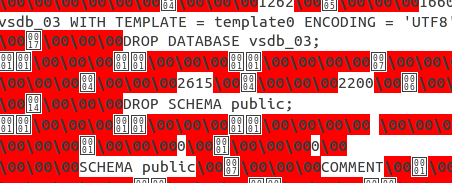
\includegraphics[width=0.5\linewidth]{pictures/content}
		\caption{Content of the file}
		\label{content}
	\end{center}
\end{figure} 
\\ \\
\textit{t tar} \\
Output a tar archive suitable for input into pg\_restore. Using this archive format allows reordering and/or exclusion of database objects at the time the database is restored. It is also possible to limit which data is reloaded at restore time.
\\ \\
\textbf{--inserts}\\
"Dump data as INSERT commands with explicit column names (INSERT INTO table (column, ...) VALUES ...). This will make restoration very slow; it is mainly useful for making dumps that can be loaded into non-PostgreSQL databases. Also, since this option generates a separate command for each row, an error in reloading a row causes only that row to be lost rather than the entire table contents." \cite{pgdumpdoc} \\
This generates the following output:
\begin{lstlisting}    
INSERT INTO mitarbeiter VALUES ('Hannah Siegel', 'HR', 'current');
INSERT INTO mitarbeiter VALUES ('Nikolaus Schrack', 'Analysten', 'current');
[..]
INSERT INTO mitarbeiter VALUES ('Aly Ahmed', 'Facility Management', 'current');
INSERT INTO mitarbeiter VALUES ('Martin Haidn', 'Managment', 'current');
INSERT INTO mitarbeiter VALUES ('Dominik Scholz', 'IT', 'current');
\end{lstlisting}    
\textbf{-t [table\_name]}\\
This option dumps only one specific table.
\subsubsection{Drop statements}
If the option \texttt{--clean} was added to the \texttt{pg\_dump} command, the triggers, tables and so on will be dropped:
\begin{lstlisting}    
DROP TRIGGER update_veranstaltung_trigger ON public.veranstaltung;
[..]
ALTER TABLE ONLY public.veranstaltung DROP CONSTRAINT pk_veranstaltung;
[..]
DROP TABLE public.veranstaltung;
[..]
DROP SEQUENCE public.logged_id_seq;
[..]
DROP FUNCTION public.update_veranstaltung();
[..]
DROP TYPE public.sync_type;
[..]
DROP EXTENSION plpgsql;
DROP SCHEMA public;
\end{lstlisting}    
\subsubsection{Performing a data restore}
Restoring from the sql file using pg\_restore didnt work at first, this was the error message:
\begin{lstlisting}    
pg\_restore: [archiver] input file appears to be a text format dump. Please use psql.
\end{lstlisting}    
Then we tried it with the file which we had generated using the \texttt{-F custom} parameter from pg\_dump.
There was no exception or anything, but somehow the import was not succesfull.
\\
\\
Happily, the restore worked with the normal sql file. All that had to be done was importing in when we were logged in in the database using the \texttt{\i filename} command.
\subsection{Physical backups}
In the Postgres Manual the following command could be found: \\
\texttt{tar -cf backup.tar /usr/local/pgsql/data} \\
But in out case we were not able to find this path. It just didn't exist.
\\ \\
"The database server must be shut down in order to get a usable backup. [..] Restoring individual tables or databases from their respective files or directories will not work because the information contained in these files is not usable without the commit log files, pg\_clog/*, which contain the commit status of all transactions.",\cite{phyback} \\
"An alternative file-system backup approach is to make a "consistent snapshot" of the data directory, if the file system supports that functionality (and you are willing to trust that it is implemented correctly). The typical procedure is to make a "frozen snapshot" of the volume containing the database, then copy the whole data directory (not just parts, see above) from the snapshot to a backup device, then release the frozen snapshot. This will work even while the database server is running. However, a backup created in this way saves the database files in a state as if the database server was not properly shut down; therefore, when you start the database server on the backed-up data, it will think the previous server instance crashed and will replay the WAL log. This is not a problem; just be aware of it (and be sure to include the WAL files in your backup). You can perform a CHECKPOINT before taking the snapshot to reduce recovery time.",\cite{phyback}
\\ \\
Other references were leading to the PGDATA folder. This folder is located at \texttt{/var/lib/postgresql/9.3/main} in our case. Still, we were not able to locate the relevant files. Pg\_dump therefore is still the better backup method in our opinion.
\subsection{Backup of Triggers / Stored Routines}
With the pg\_dump command, triggers and functions had been restored as well.
\subsection{Remote Backups}
The pg\_dump method has a parameter -h in which an host can be specified. Therefore it enables a remote host backup.
\subsection{Online Backups}
The pg\_dump method enables online backups.
With an physical method, the database server must be shut down in order to get a usable backup.
\subsection{Automated Backups}
First, we downloaded an .sh file from \cite{autppg}. It basically is the same file as the automysqlbackup, but customised for PostgreSQL. \\
We put the file into the \texttt{/home/hsiegel/Documents/sync\_het\_db} folder and we added the following line to our crontab (using the \texttt{crontab -e} command, just as before). 
\begin{lstlisting}    
40 15 * * * /home/hsiegel/Documents/sync_het_db/autopgbackup.sh
\end{lstlisting}    
In order to get this working, we had to change the Database names in the script from all to the ones we wanted to backup, because otherwise it wouldn't work. As it can be seen in figure \ref{fig:b1}, the backup happened at exactly 15:40. The database vsdb\_03 has been successfully backuped (figure \ref{fig:b2}).  
\begin{figure}[!h]
	\begin{center}
		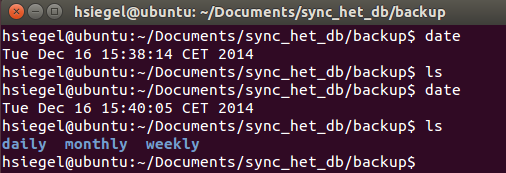
\includegraphics[width=0.5\linewidth]{pictures/pgbackupaut}
		\caption{Time of the backup}
		\label{fig:b1}
	\end{center}
\end{figure} 
\begin{figure}[!h]
	\begin{center}
		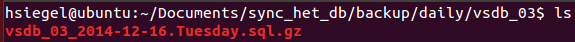
\includegraphics[width=0.5\linewidth]{pictures/pgbackupaut2}
		\caption{Content of the backup folder}
		\label{fig:b2}
	\end{center}
\end{figure} 
\newpage
\section{Summary}
After having tried out all the possible backup methods, we finally can conclude, that the mysql\_dump and the pg\_dump were the best tools. \\ 
This was because the logical files were better readable, and it was easier doing the backup. The two tools provide the user with a wide range of possibilities. \\
Automated backups should be done using the cron-deamon. We liked this option, because it was really easy and it also provides a lot of functionality. Besides this, the crontab was a centralized place in which we had both the mysql and the postgres backup and therefore it would be easy to change both of them at the same time.

\section{Problems}
\textbf{Mysql connection didn't work out} \\
When trying to connect to the mysql Database, the following error was thrown:
\texttt{ERROR 2002 (HY000): Can't connect to local MySQL server through socket '/var/run/mysqld/mysqld.sock'} \\
The following steps had to be done: \\
\\ 
\begin{enumerate}
\item Super user or sudo should be used. (\texttt{sudo su}) 
\item The file \texttt{/etc/mysql/my.cnf} must be opened 
\item The bind address had to be changed to \texttt{127.0.0.1}
\item Then \texttt{service mysql restart} must be executed
\end{enumerate}
\cite{mysqlProblem1}

http://www.pgadmin.org/docs/1.8/pgagent-install.html
\newpage
\begin{thebibliography}{56}

  
 \bibitem{mysqlProblem1} 
  \textbf{ERROR 2002: Can't connect to local MySQL server through socket \\ StackOverflow} \\ Peter Mortensen Apr 13 at 10:45 and  rshahriar Oct 11 '12 at 6:27 \\
  \textit{http://stackoverflow.com/questions/11657829/error-2002-hy000-cant-connect-to-local-mysql-server-through-socket-var-run}
  \newline last used: 2014.12.05, 13:15
 
 \bibitem{mysqldumpman} 
  \textbf{Mysql Manual 5.5}, mysqldump — A Database Backup Program\\
  \textit{http://dev.mysql.com/doc/refman/5.5/en/mysqldump.html}
  \newline last used: 2014.12.05, 13:55
    
  \bibitem{mysqlbackupandrectypesman} 
  \textbf{Mysql Manual 5.5} Backup and Recovery Types\\
  \textit{http://dev.mysql.com/doc/refman/5.5/en/backup-types.html}
  \newline last used: 2014.12.06, 19:01
  
  \bibitem{mysqlenterprisebackup} 
  \textbf{Mysql Website}MySQL Enterprise Backup\\
  \textit{http://www.mysql.com/products/enterprise/backup.html}
  \newline last used: 2014.12.08, 10:49

  \bibitem{so1} 
  \textbf{StackOverflow}, RolandoMySQLDBA - answered Mar 7 '12 at 17:45 St\\
  \textit{http://serverfault.com/questions/367255/linux-mysql-is-it-safe-to-copy-mysql-db-files-with-cp-command-from-one-db-to
}
  \newline last used: 2014.12.08, 11:39


 \bibitem{mysqlhotcopyman} 
  \textbf{Mysql Manual 5.5} mysqlhotcopy — A Database Backup Program\\
  \textit{http://dev.mysql.com/doc/refman/5.5/en/mysqlhotcopy.html}
  \newline last used: 2014.12.08, 14:16

 \bibitem{mysqlhtcoptut} 
  \textbf{Backup and Restore MySQL Database using mysqlhotcopy},  Ramesh Natarajan \\
  \textit{http://www.thegeekstuff.com/2008/07/backup-and-restore-mysql-database-using-mysqlhotcopy/}
  \newline last used: 2014.12.08, 14:44
  
  \bibitem{balbalbla} 
  \textbf{How To Backup MySQL Databases on an Ubuntu VPS},  Justin Ellingwood \\
  \textit{https://www.digitalocean.com/community/tutorials/how-to-backup-mysql-databases-on-an-ubuntu-vps}
  \newline last used: 2014.12.08, 15:30
  


   \bibitem{sceduleddbbck} 
  \textbf{Scheduled DB backup with automysqlbackup}, January 5, 2013 \\
  \textit{https://pelanne.com/blog/scheduled-db-backup-automysqlbackup/}
  \newline last used: 2014.12.10, 09:33
  
   \bibitem{uglywebpage} 
  \textbf{Creating MySQL Backups With AutoMySQLBackup On Ubuntu 9.10}\\ Falko Timme, January 27, 2010 \\
  \textit{http://www.howtoforge.com/creating-mysql-backups-with-automysqlbackup-on-ubuntu-9.10}
  \newline last used: 2014.12.10, 09:35
  
  
   \bibitem{crontabref} 
  \textbf{Crontab – Quick Reference}  Hemant Sharma \\
  \textit{http://www.adminschoice.com/crontab-quick-reference}
  \newline last used: 2014.12.14, 15:59
  
    \bibitem{pgdumpdoc} 
  \textbf{Postgres Documentation} SQL Dump\\
  \textit{http://www.postgresql.org/docs/9.1/static/backup-dump.html}
  \newline last used: 2014.12.14, 19:32
    
    \bibitem{pgdoc2} 
  \textbf{Postgres Documentation} pg\_restore\\
  \textit{  http://www.postgresql.org/docs/9.1/static/app-pgrestore.html}
  \newline last used: 2014.12.14, 20:03

    \bibitem{automysql} 
  \textbf{bjoerne.com} 4. September 2013\\
  \textit{http://www.bjoerne.com/mysql-backups-mit-automysqlbackup-erstellen/}
  \newline last used: 2014.12.15, 15:16

    \bibitem{autppg} 
  \textbf{Autobackup Postgres Script}Aaron Axelsen, 2005 4. September 2013\\
  \textit{http://autopgsqlbackup.frozenpc.net}
  \newline last used: 2014.12.15, 15:17
  
  \bibitem{phyback} 
  \textbf{PostgreSQL 9.3 Documentation} Chapter 24. Backup and Restore	\\
  \textit{http://www.postgresql.org/docs/9.3/static/backup-file.html}
  \newline last used: 2014.12.15, 16:39
	
	
	
\end{thebibliography}
\end{document}
%\todo{INKREMENTELLE BACKUPS MYSQL?????}
%Online Backup Postgres
%Physical backup Postgres

% TODO mysql 20:15 testen!!!!!